% Options for packages loaded elsewhere
\PassOptionsToPackage{unicode}{hyperref}
\PassOptionsToPackage{hyphens}{url}
%
\documentclass[
]{article}
\usepackage{amsmath,amssymb}
\usepackage{lmodern}
\usepackage{iftex}
\ifPDFTeX
  \usepackage[T1]{fontenc}
  \usepackage[utf8]{inputenc}
  \usepackage{textcomp} % provide euro and other symbols
\else % if luatex or xetex
  \usepackage{unicode-math}
  \defaultfontfeatures{Scale=MatchLowercase}
  \defaultfontfeatures[\rmfamily]{Ligatures=TeX,Scale=1}
\fi
% Use upquote if available, for straight quotes in verbatim environments
\IfFileExists{upquote.sty}{\usepackage{upquote}}{}
\IfFileExists{microtype.sty}{% use microtype if available
  \usepackage[]{microtype}
  \UseMicrotypeSet[protrusion]{basicmath} % disable protrusion for tt fonts
}{}
\makeatletter
\@ifundefined{KOMAClassName}{% if non-KOMA class
  \IfFileExists{parskip.sty}{%
    \usepackage{parskip}
  }{% else
    \setlength{\parindent}{0pt}
    \setlength{\parskip}{6pt plus 2pt minus 1pt}}
}{% if KOMA class
  \KOMAoptions{parskip=half}}
\makeatother
\usepackage{xcolor}
\usepackage[margin=1in]{geometry}
\usepackage{graphicx}
\makeatletter
\def\maxwidth{\ifdim\Gin@nat@width>\linewidth\linewidth\else\Gin@nat@width\fi}
\def\maxheight{\ifdim\Gin@nat@height>\textheight\textheight\else\Gin@nat@height\fi}
\makeatother
% Scale images if necessary, so that they will not overflow the page
% margins by default, and it is still possible to overwrite the defaults
% using explicit options in \includegraphics[width, height, ...]{}
\setkeys{Gin}{width=\maxwidth,height=\maxheight,keepaspectratio}
% Set default figure placement to htbp
\makeatletter
\def\fps@figure{htbp}
\makeatother
\setlength{\emergencystretch}{3em} % prevent overfull lines
\providecommand{\tightlist}{%
  \setlength{\itemsep}{0pt}\setlength{\parskip}{0pt}}
\setcounter{secnumdepth}{-\maxdimen} % remove section numbering
\ifLuaTeX
  \usepackage{selnolig}  % disable illegal ligatures
\fi
\IfFileExists{bookmark.sty}{\usepackage{bookmark}}{\usepackage{hyperref}}
\IfFileExists{xurl.sty}{\usepackage{xurl}}{} % add URL line breaks if available
\urlstyle{same} % disable monospaced font for URLs
\hypersetup{
  pdftitle={gibbs\_sampling\_and\_random\_walk},
  pdfauthor={Yijin Wang},
  hidelinks,
  pdfcreator={LaTeX via pandoc}}

\title{gibbs\_sampling\_and\_random\_walk}
\author{Yijin Wang}
\date{2023-04-30}

\begin{document}
\maketitle

Given the fact that we can easily identify the distribution that most of
the conditional posteriors follows, we choose to use Gibbs sampling.
Gibbs sampling is an efficient sampler to create approximated data that
follows a target joint distribution with several conditional
distributions. It is a sequential approach that updates parameter value
one by one with information of other parameters.

Still, we could not find a regular distribution that has the density
function that matches with the conditional posterior of \(\sigma^2\).
Therefore, we incorporated Metropolis Hasting Random Walk into Gibbs
sampling. Metropolis Hasting Random Walk finds approximated values of
\(\sigma^2\) by accepting and rejecting proposed value with an
acceptance probability that helps retain balance of the system. In our
algorithm, we worked with log-scaled posterior values instead of the
original-scaled posterior because \(\frac{1}{\sigma^N}\) dominates the
entire posterior value where \(N\) is the total number of observations
in the dataset.

In our investigation of hurricane wind speed, we used Gibbs sampling and
as Metropolis Hasting Random Walk as the following:

\begin{figure}
\centering
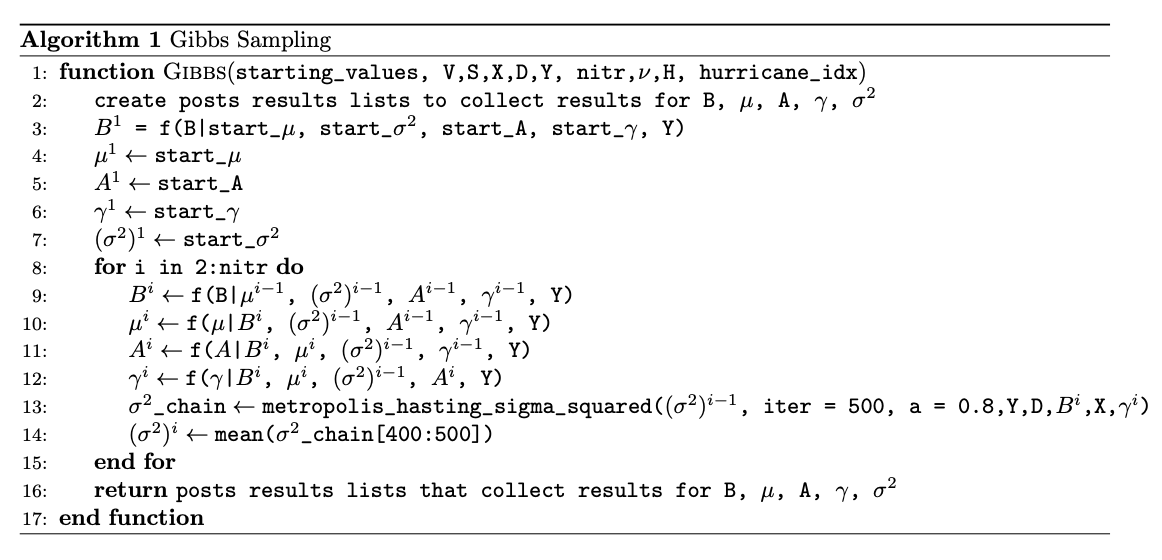
\includegraphics{algo_fig/gibbs_sampling.png}
\caption{Gibbs Sampling}
\end{figure}

\begin{figure}
\centering
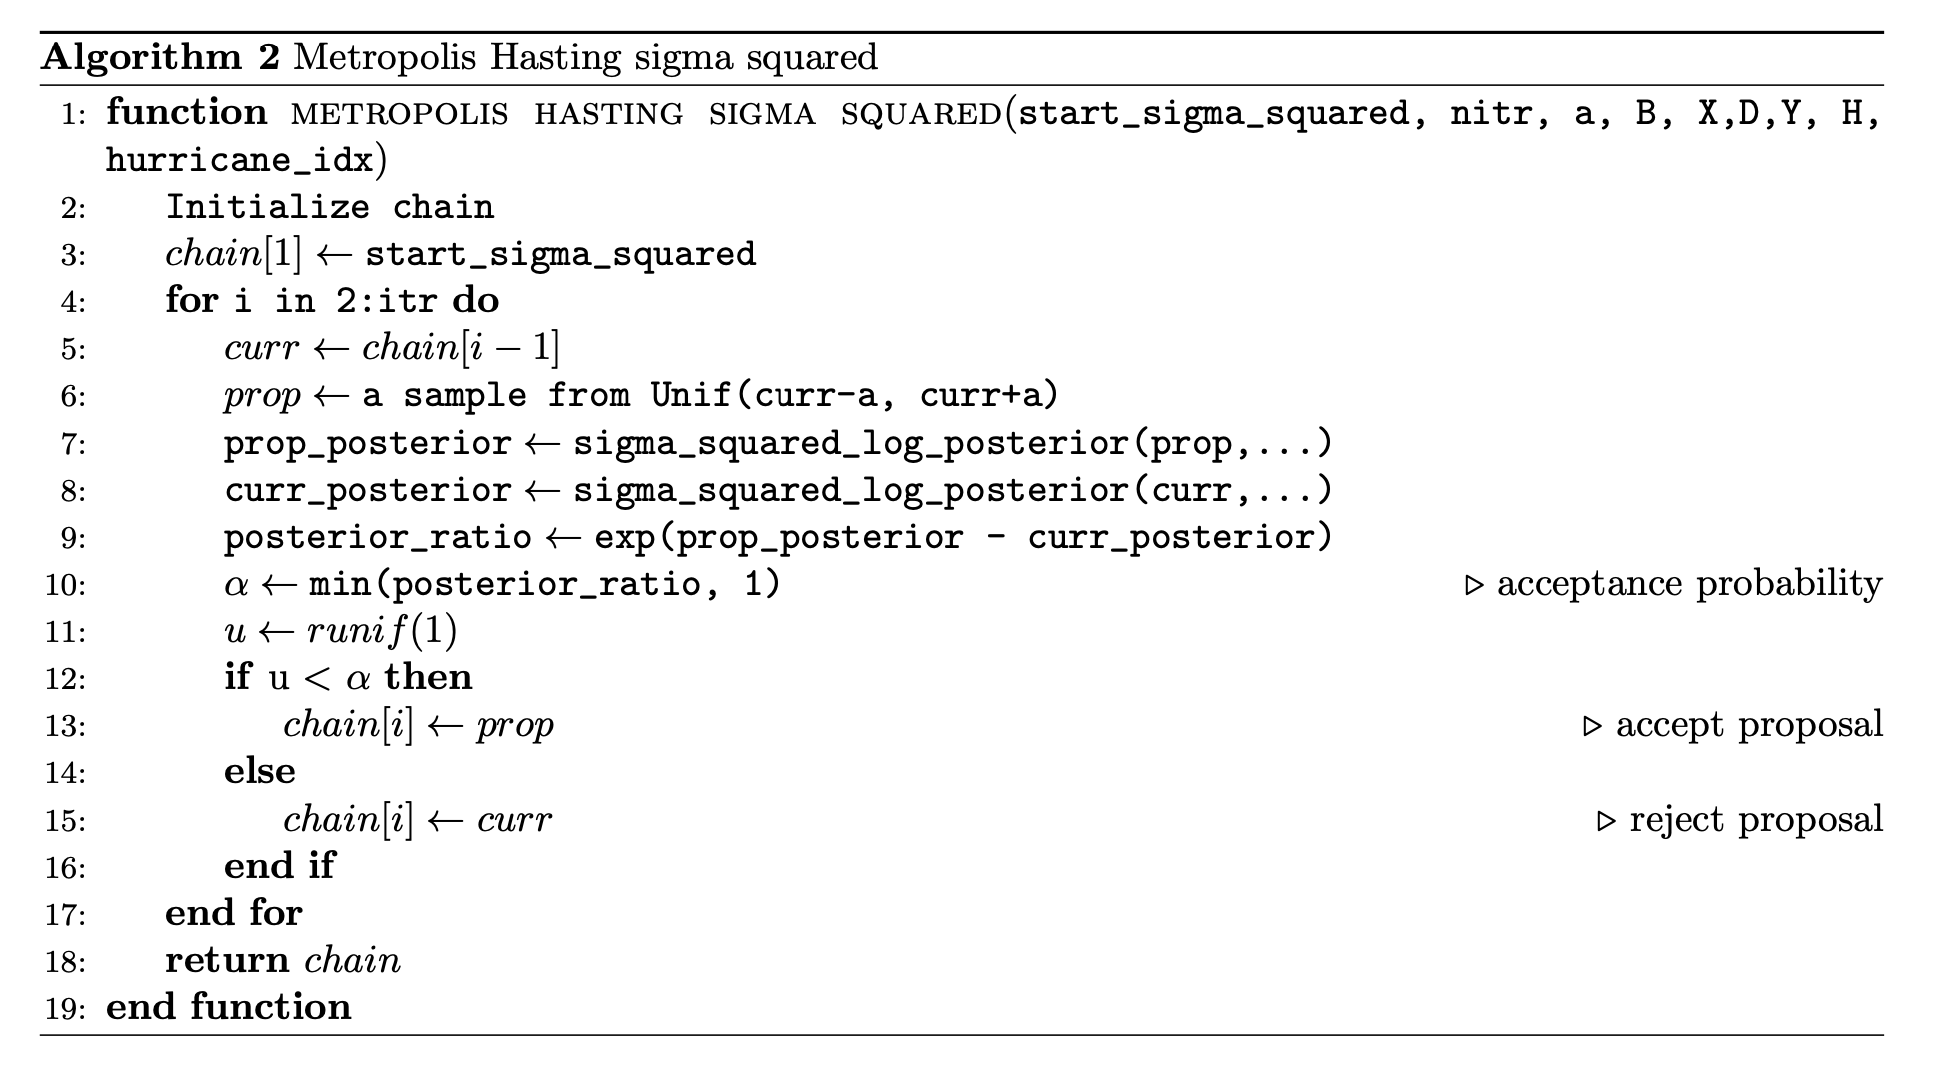
\includegraphics{algo_fig/random_walk.png}
\caption{Metropolis Hasting Random Walk}
\end{figure}

\end{document}
